\documentclass{ctexart}  
\usepackage[left=2cm,right=1.97cm,top=2cm,bottom=2cm]{geometry}	
\usepackage{ctex}
\usepackage{palatino}
\usepackage{lipsum}
\usepackage{graphicx}
\usepackage{hyperref}
\usepackage{tabularray}
\usepackage{color}
\usepackage{listings}
\usepackage{float}
\usepackage{xcolor}
\usepackage[longtable]{multirow}
\usepackage{longtable}
\title{\heiti \zihao{2}实验三:命令行环境、Python入门基础、
Python视觉应用学习实验报告}
\author{\kaishu \zihao{-4} 邓林\qquad 23020007014\\
\songti \zihao{-5}中国海洋大学 \qquad 23软件工程 }
\date{}
\ctexset{section={format={\heiti \zihao{4}}},
subsection={format={ \songti \zihao{4}},beforeskip=0pt,afterskip=0pt},
subsubsection={format={\kaishu \zihao{4}},beforeskip=0pt ,afterskip=0pt}}
%%%%%%%%%%%%%%%%%%%%%%%%%

\begin{document}
    \maketitle
\vspace{-20pt}\begin{abstract}				
    本实验报告主要记录了作者通过课程网站及B站学习命令行环境、Python入门基础、
    Python视觉应用的学习过程以及心得。
\end{abstract}

\section{实验内容}
1. 命令行环境\\
\begin{longtable}{c|cl}
    \hline
    \multicolumn{3}{c}{命令行环境(tumx)}                                                                     \\* 
    \hline
    \multirow{5}{*}{会话} & tmux                                      & 开始一个新的会话                          \\*
                        & tmux new -s NAME                          & 以指定名称开始一个新的会话                     \\*
                        & tmux ls                                   & 列出当前所有会话                          \\*
                        & C-b d                                     & 将当前会话分离                           \\*
                        & tmux a                                    & 重新连接最后一个会话                        \\* 
    \hline
    \multirow{6}{*}{窗口} & C-b c                                     & 创建一个新的窗口,使用~C-d~关闭                \\*
                        & C-b N                                     & 跳转到第~\textit{N}~个窗口,注意每个窗口都是有编号的  \\*
                        & C-b p                                     & 切换到前一个窗口                          \\*
                        & C-b n                                     & 切换到下一个窗口                          \\*
                        & C-b ,                                     & 重命名当前窗口                           \\*
                        & C-b w                                     & 列出当前所有窗口                          \\* 
    \hline
    \multirow{6}{*}{面板} & C-b "                                     & 水平分割                              \\*
                        & C-b \%                                    & 垂直分割                              \\*
                        & C-b 方向                                    & 切换到指定方向的面板,方向 指的是键盘上的方向键          \\*
                        & C-b z                                     & 切换当前面板的缩放                         \\*
                        & \textless{}C-b\textgreater{} {[}~开始往回卷动屏幕 & 按下空格键来开始选择,回车键复制选中的部分             \\*
                        & C-b 空格                                    & 在不同的面板排布间切换                       \\
    \hline
    \end{longtable}

    2. Python入门基础\\
    \begin{longtable}{c|l}
        \hline
        \multicolumn{2}{c}{Python}                                                                                                                    \endfirsthead 
        \hline
        \begin{tabular}[c]{@{}c@{}}print(内容,内容,...,内容,sep="内容",end="内容")\\sep空则输出" ",end为空则输出"\textbackslash{}n"\end{tabular} & 输出语句                  \\
        变量=input("输入提示")                                                                                                      & 输入语句,赋值语句             \\
        \begin{tabular}[c]{@{}c@{}}if condition:\\elif condition:\\else:\end{tabular}                                         & if 语句                 \\
        and                                                                                                                   &                       \\
        or                                                                                                                    & \textbar{}\textbar{}  \\
        not                                                                                                                   & !                     \\
        \begin{tabular}[c]{@{}c@{}}a in [1,变量,"内容"]\\a in \{"内容1":100,"内容2":1\}\end{tabular}                                  & 条件判断语句                \\
        a in "字符串"                                                                                                            & 条件判断语句                \\
        变量1=变量2.upper()                                                                                                       & 转大写                   \\
        变量1=变量2.lower()                                                                                                       & 转小写                   \\
        变量1=len(变量2)                                                                                                          & 取长度                   \\
        变量="X:\{0\},Y:\{1\}".format(变量1,变量2)                                                                                  & 赋值语句                  \\
        \hline
        \end{longtable}
        
        3. Python视觉设计\\
        \begin{longtable}{cl} 
            \hline
            \multicolumn{2}{c}{Python视觉应用}                                                                                                                           \endfirsthead 
            \hline
            image = cv2.imread("图片路径")                                         & 获取图片存放在image变量中                                                                     \\
            cv2.namedWindow("image",~cv2.WINDOW\_NORMAL)                       & 设置可调整大小的窗口                                                                          \\
            cv2.imshow("image", image)                                         & 显示image中存放的图片                                                                       \\
            cv2.resizeWindow("image", 800, 1000)                               & 调整窗口大小                                                                              \\
            cv2.waitKey()                                                      & 等待用户按键事件                                                                            \\
            cv2.imshow("blue",image[:,:,0])                                    & \begin{tabular}[c]{@{}l@{}}将蓝色通道的数据以图像的形式显示在指定名称为\\"blue"的窗口中\end{tabular}          \\
            cv2.imshow("green",image[:,:,1])                                   & \begin{tabular}[c]{@{}l@{}}将绿色通道的数据以图像的形式显示在指定名称为\\"green"的窗口中\end{tabular}         \\
            cv2.imshow("red",image[:,:,2])                                     & \begin{tabular}[c]{@{}l@{}}将红色通道的数据以图像的形式显示在指定名称为\\"red"的窗口中\end{tabular}           \\
            grey = cv2.cvtColor(image,cv2.COLOR\_BGR2GRAY)                     & 创建灰度图                                                                               \\
            crop = image[长1:长2, 宽1:宽2]                                         & 截取图片                                                                                \\
            resized\_crop = cv2.resize(crop, (1000, 800))                      & 调整图片大小                                                                              \\
            image = np.zeros([300, 300, 3], dtype=np.uint8)                    & \begin{tabular}[c]{@{}l@{}}创建了一个 300×300 且具有 3 个颜色通道、元素\\值全为 0的图像数据结构\end{tabular}  \\
            cv2.line(image,(100, 200),(250,250),(255, 0, 0), 2)                & 绘制线段                                                                                \\
            cv2.rectangle(image, (30, 100),(60, 150), (0, 255, 0), 2)          & 绘制矩形                                                                                \\
            cv2.circle(image, (150, 100), 20, (0, 0, 255), 3)                  & 绘制圆                                                                                 \\
            cv2.putText(image, "hello", (100,50), 0, 1, (255,~~255,255),~2, 1) & 绘制文字                                                                                \\
            \hline
            \end{longtable}
\subsection{命令行环境}
\begin{enumerate}
\item 暂停和后台执行进程\\
信号可以让进程做其他的事情,而不仅仅是终止它们。

我们可以使用 fg 或 bg 命令恢复暂停的工作。它们分别表示在前台继续或在后台继续。

jobs 命令会列出当前终端会话中尚未完成的全部任务。使用 pid 引用这些任务(也可以用 pgrep 找出 pid)。更加符合直觉的操作是您可以使用百分号 + 任务编号(jobs 会打印任务编号)来选取该任务。如果要选择最近的一个任务,可以使用 \$! 这一特殊参数。

命令中的 \& 后缀可以让命令在直接在后台运行,可以直接在 shell 中继续做其他操作。

让已经在运行的进程转到后台运行,可以键入 Ctrl-Z ,然后紧接着再输入 bg。注意,后台的进程仍然是您的终端进程的子进程,一旦您关闭终端(会发送另外一个信号 SIGHUP),这些后台的进程也会终止。为了防止这种情况发生,可以使用 nohup(一个用来忽略 SIGHUP 的封装)来运行程序。针对已经运行的程序,可以使用 disown 。

\item 终端多路复用\\
tmux 这类的终端多路复用器可以允许我们基于面板和标签分割出多个终端窗口,这样便可以同时与多个 shell 会话进行交互。
\item 别名\\
alias alias\_name="command\_to\_alias arg1 arg2"\\
注意, = 两边是没有空格的,因为 alias 是一个 shell 命令,它只接受一个参数。

\item 配置文件(Dotfiles)\\
对于 bash 来说,在大多数系统下,可以通过编辑 .bashrc 或 .bash\_profile 来进行配置。
\begin{itemize}
    \item bash \~/.bashrc, \~/.bash\_profile
    \item git - \~/.gitconfig
    \item vim - \~/.vimrc 和 \~/.vim 目录
    \item ssh - \~/.ssh/config
    \item tmux - \~/.tmux.conf
\end{itemize}
\begin{figure}[H]
    \centering
    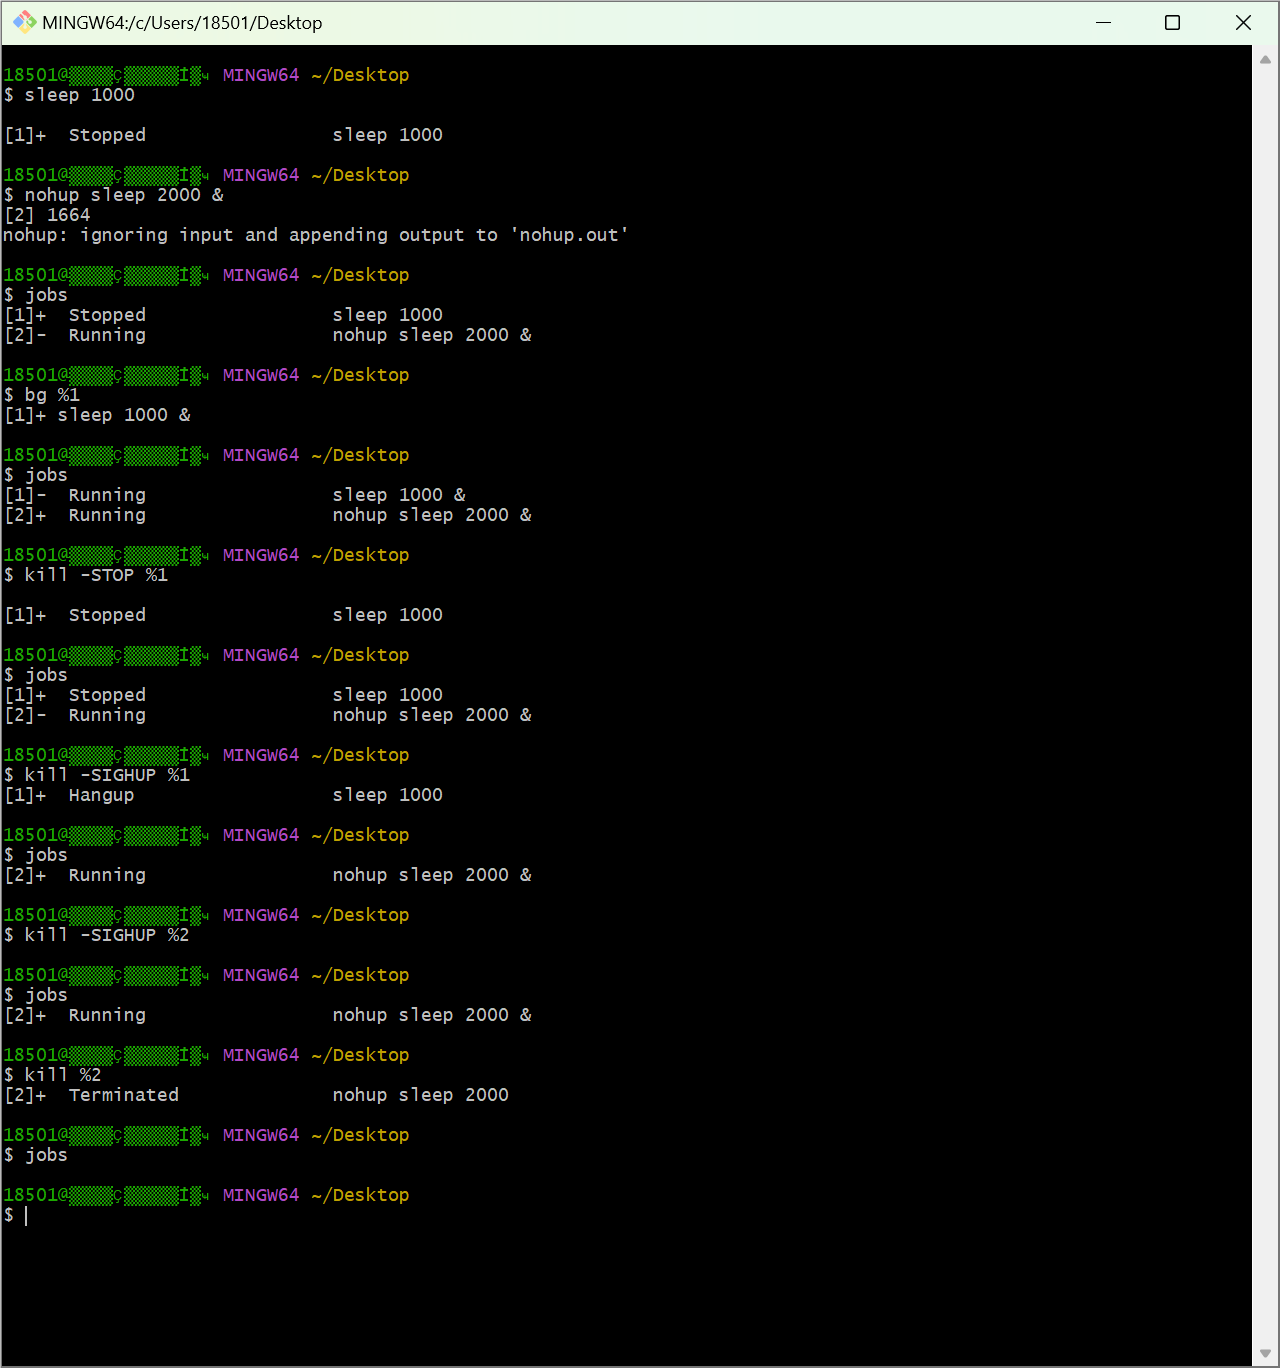
\includegraphics[width=14cm]{f485e444333525133ef9f155fe3f6593.png}
    \caption{操作如图}
    \label{fig:2}
\end{figure}
\item 远端设备\\
通过 SSH 复制文件\\
scp:当需要拷贝大量的文件或目录时,使用 scp 命令则更加方便,因为它可以方便的遍历相关路径。语法如下:\\
scp path/to/local\_file remote\_host:path/to/remote\_file\\
rsync 对 scp 进行了改进,它可以检测本地和远端的文件以防止重复拷贝。它还可以提供一些诸如符号连接、权限管理等精心打磨的功能。甚至还可以基于 --partial 标记实现断点续传。rsync 的语法和 scp 类似。

\end{enumerate}

\subsection{Python入门基础}


\subsection{Python视觉应用}

\section{课后习题}
\subsection{命令行环境}
\begin{enumerate}
    \item 在终端中执行 sleep 10000 这个任务。然后用 Ctrl-Z 将其切换到后台并使用 bg 来继续允许它。
    现在,使用 pgrep 来查找 pid 并使用 pkill 结束进程而不需要手动输入 pid。
\begin{figure}[H]
    \centering
    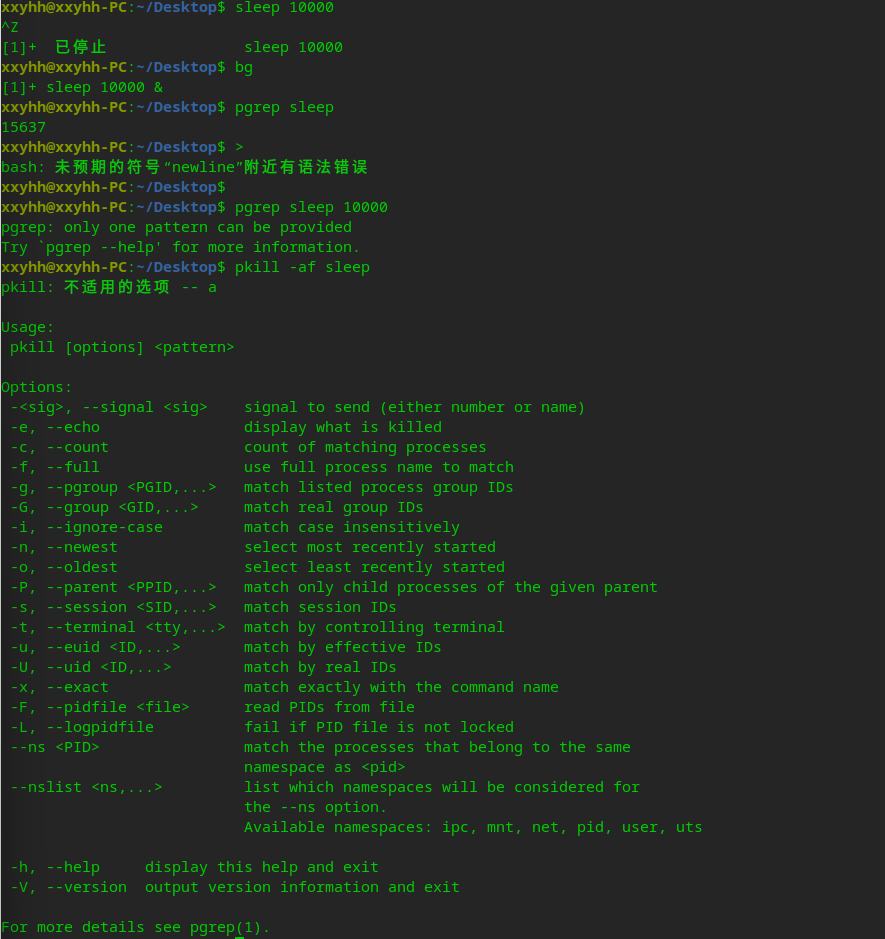
\includegraphics[width=14cm]{2483d6ccf68524e32c1d10cc130e50de.png}
    \caption{课后第1.1题如图}
    \label{fig:10}
\end{figure}

    \item 在这个练习中,我们使用 sleep 60 \& 作为先执行的程序。
    一种方法是使用 wait 命令。尝试启动这个休眠命令,然后待其结束后再执行 ls 命令。
    \begin{figure}[H]
        \centering
        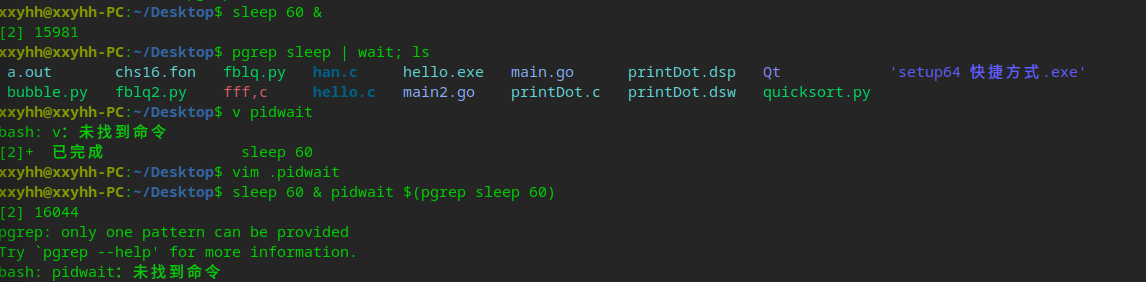
\includegraphics[width=14cm]{f5b857233ad1ad2d039067550ba35c06.png}
        \caption{课后第1.2题如图}
        \label{fig:8}
    \end{figure}


\item tmux 是一个高度可定制的工具,可以使用相关快捷键创建多个标签页并在它们间导航。

\begin{figure}[H]
    \centering
    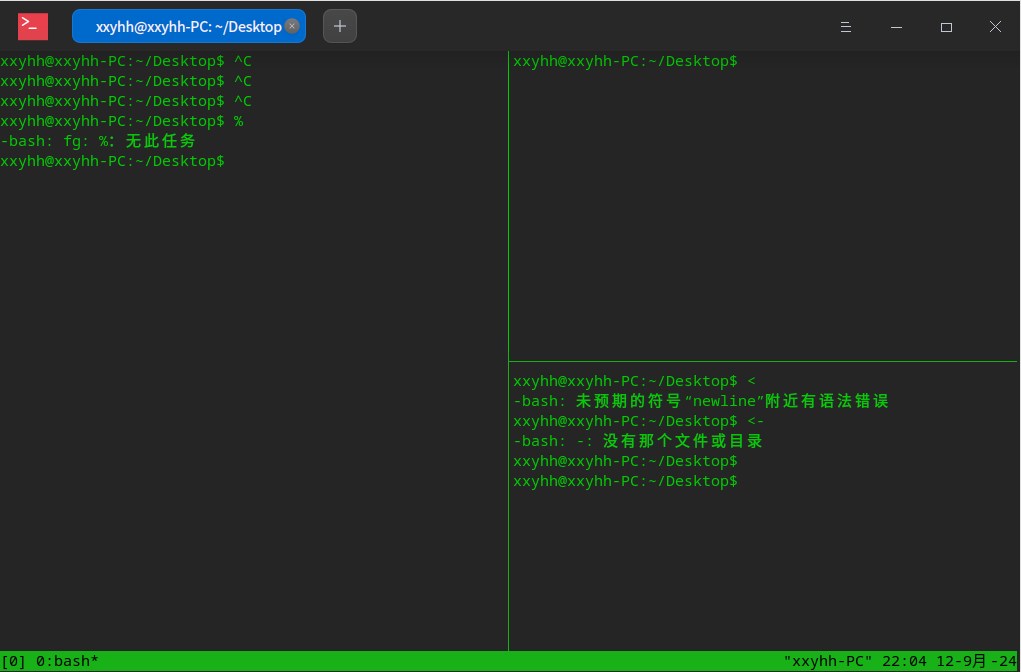
\includegraphics[width=14cm]{25ab931818a960c8606f757cf1b15eff.png}
    \caption{课后第2题如图}
    \label{fig:6}
\end{figure}

\item 别名\\
1. 创建一个 dc 别名,它的功能是当我们错误的将 cd 输入为 dc 时也能正确执行。\\
2. 执行 history | awk '{\$1="";print substr(\$0,2)}' | sort | uniq -c | sort -n | tail -n 10 
来获取最常用的十条命令,尝试为它们创建别名。
\begin{figure}[H]
    \centering
    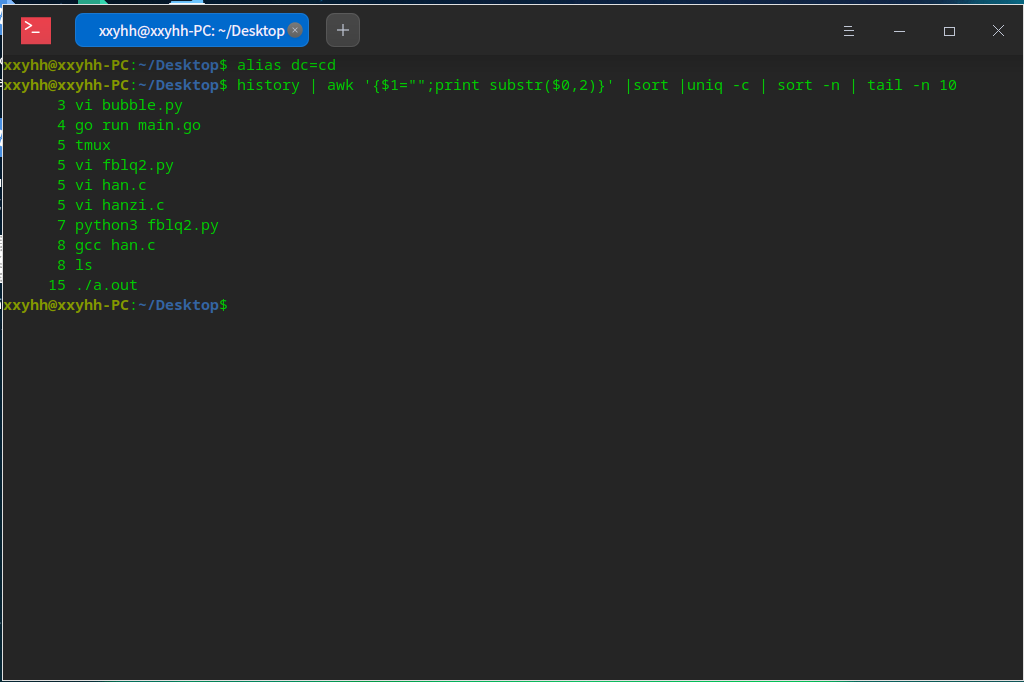
\includegraphics[width=14cm]{dcb450f12a9c1cff67bbd67c16c58d2b.png}
    \caption{课后第2题如图}
    \label{fig:7}
\end{figure}
\end{enumerate}
\section{练习实例}
\subsection{Python入门基础}
以下为用Python语法编写的游戏代码展示:\\
\begin{figure}[H]
    \centering
    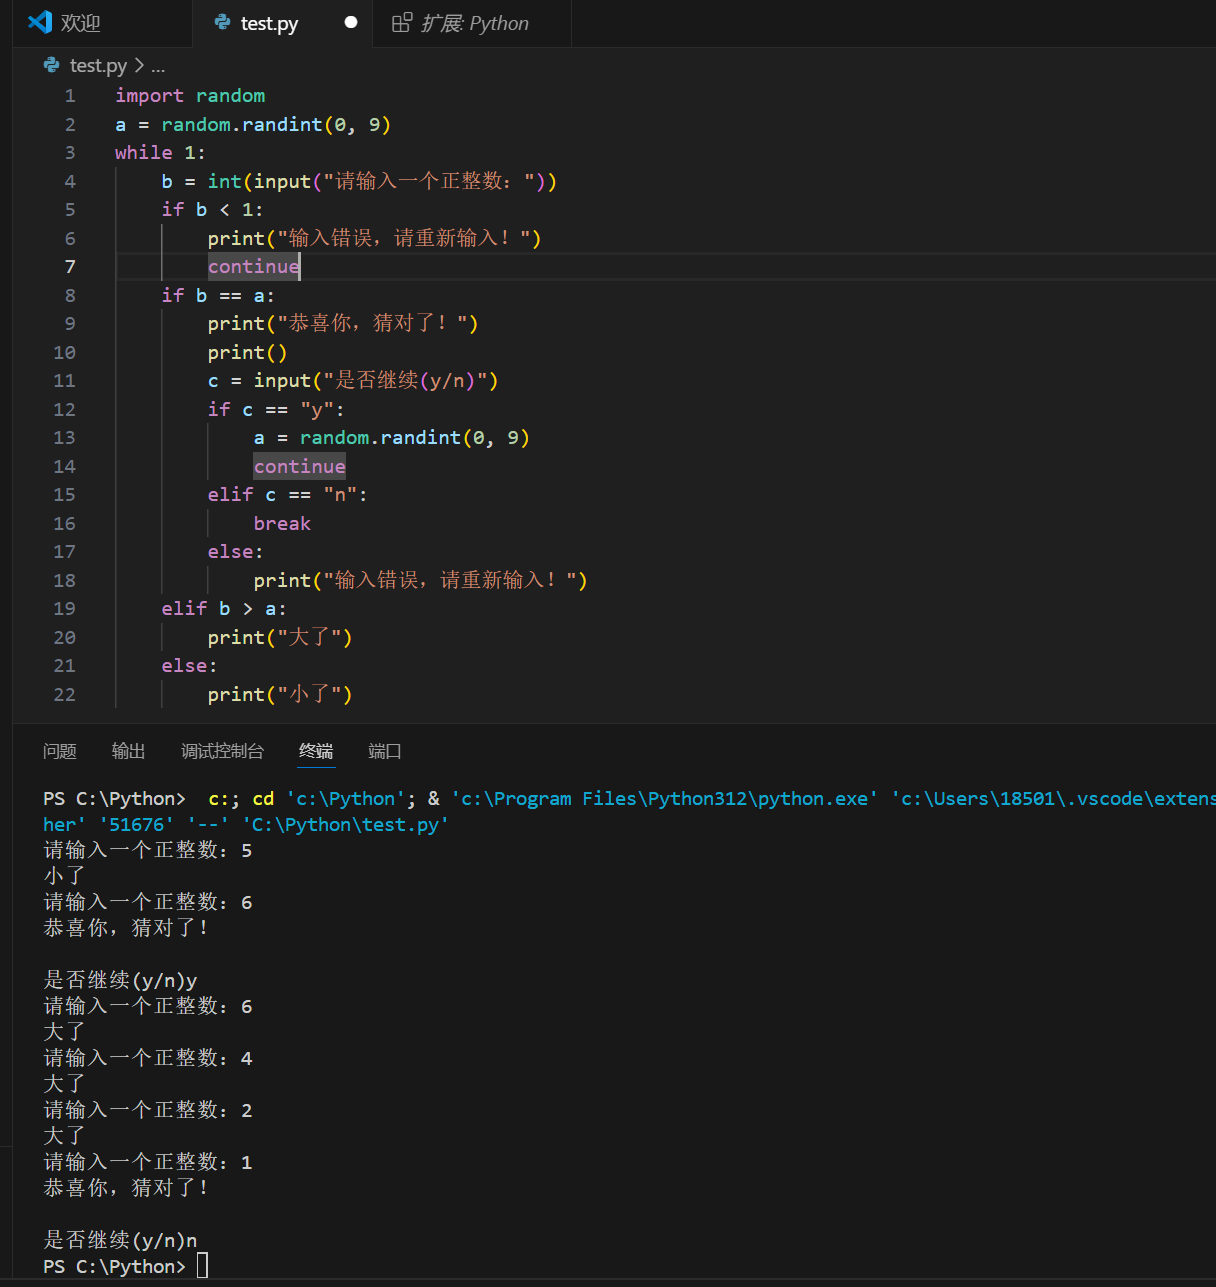
\includegraphics[width=12cm]{dc30954917dbdb9ff42e049b4c26fc44.png}
    \caption{猜数字游戏代码}
    \label{fig:11}
\end{figure}
应用了输入输出语句,if语句,while语句,random生成随机数
\subsection{Python视觉应用}
\begin{enumerate}
    \item 显示图片
    \begin{figure}[H]
        \centering
        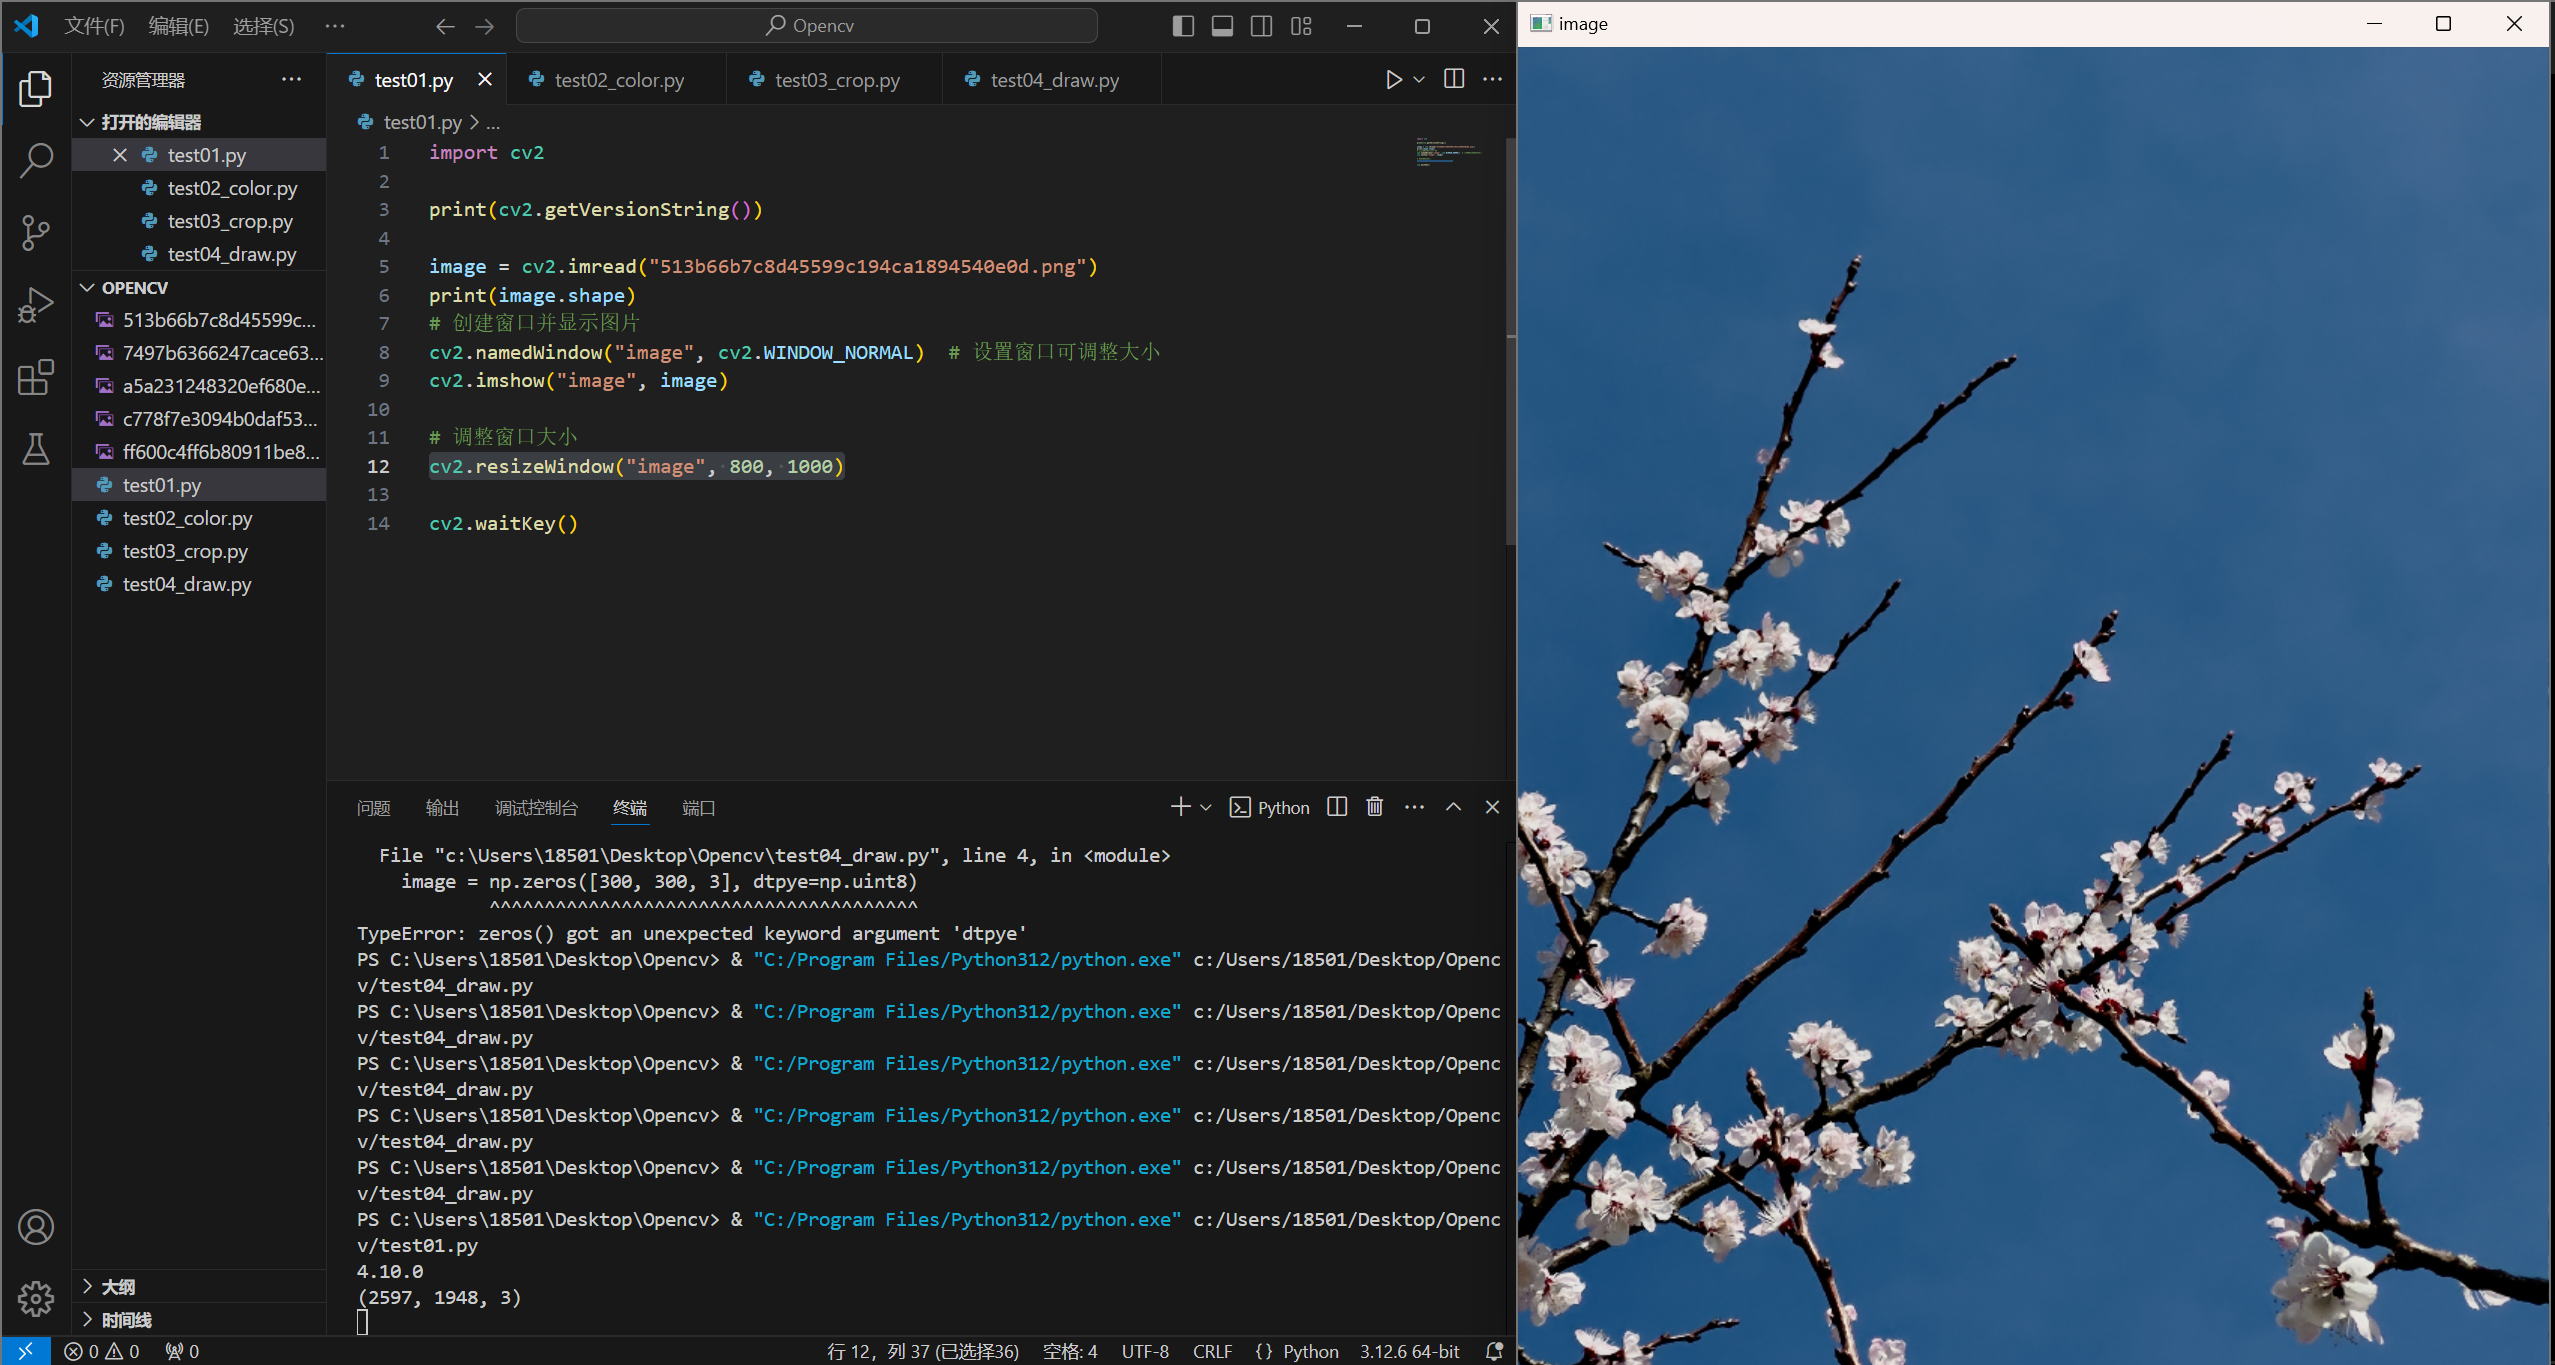
\includegraphics[width=12cm]{bae69f4cc4273bbe5c67937cac4577a4.png}
        \caption{如图}
        \label{fig:1}
    \end{figure}

    \item 显示三色图及灰度图
    \begin{figure}[H]
        \centering
        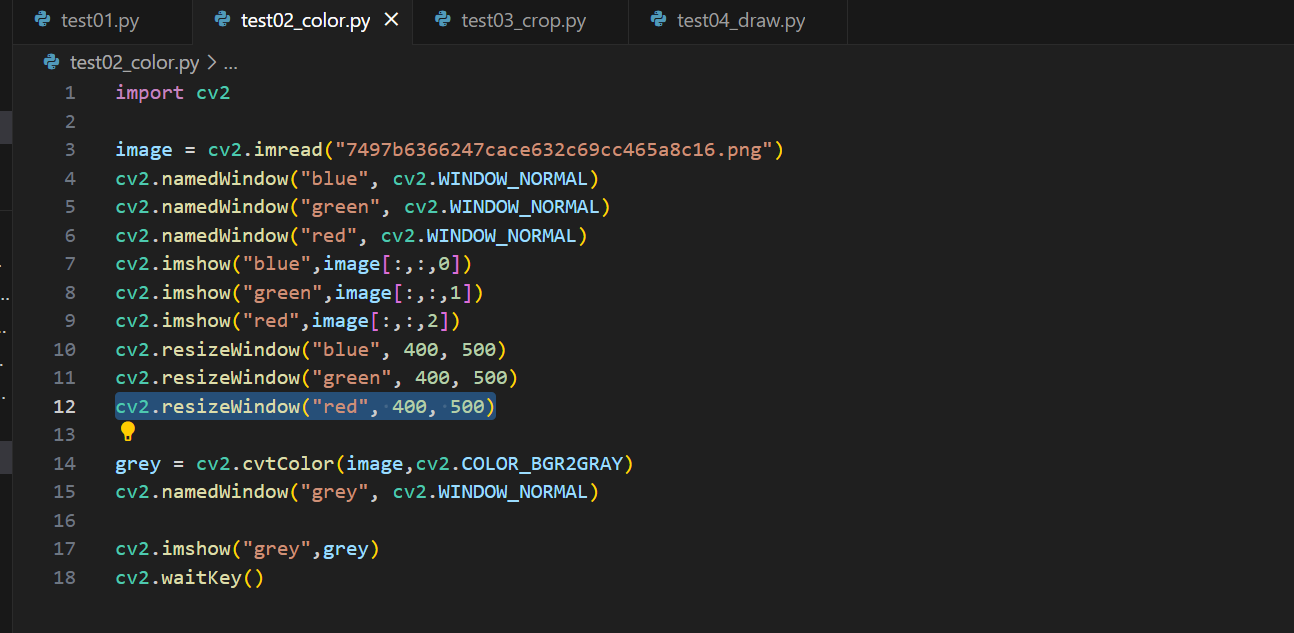
\includegraphics[width=14cm]{f53ae908c9fa737a22919eca1122cd49.png}
        \caption{代码}
        \label{fig:1}
    \end{figure}
    \begin{figure}[H]
        \centering
        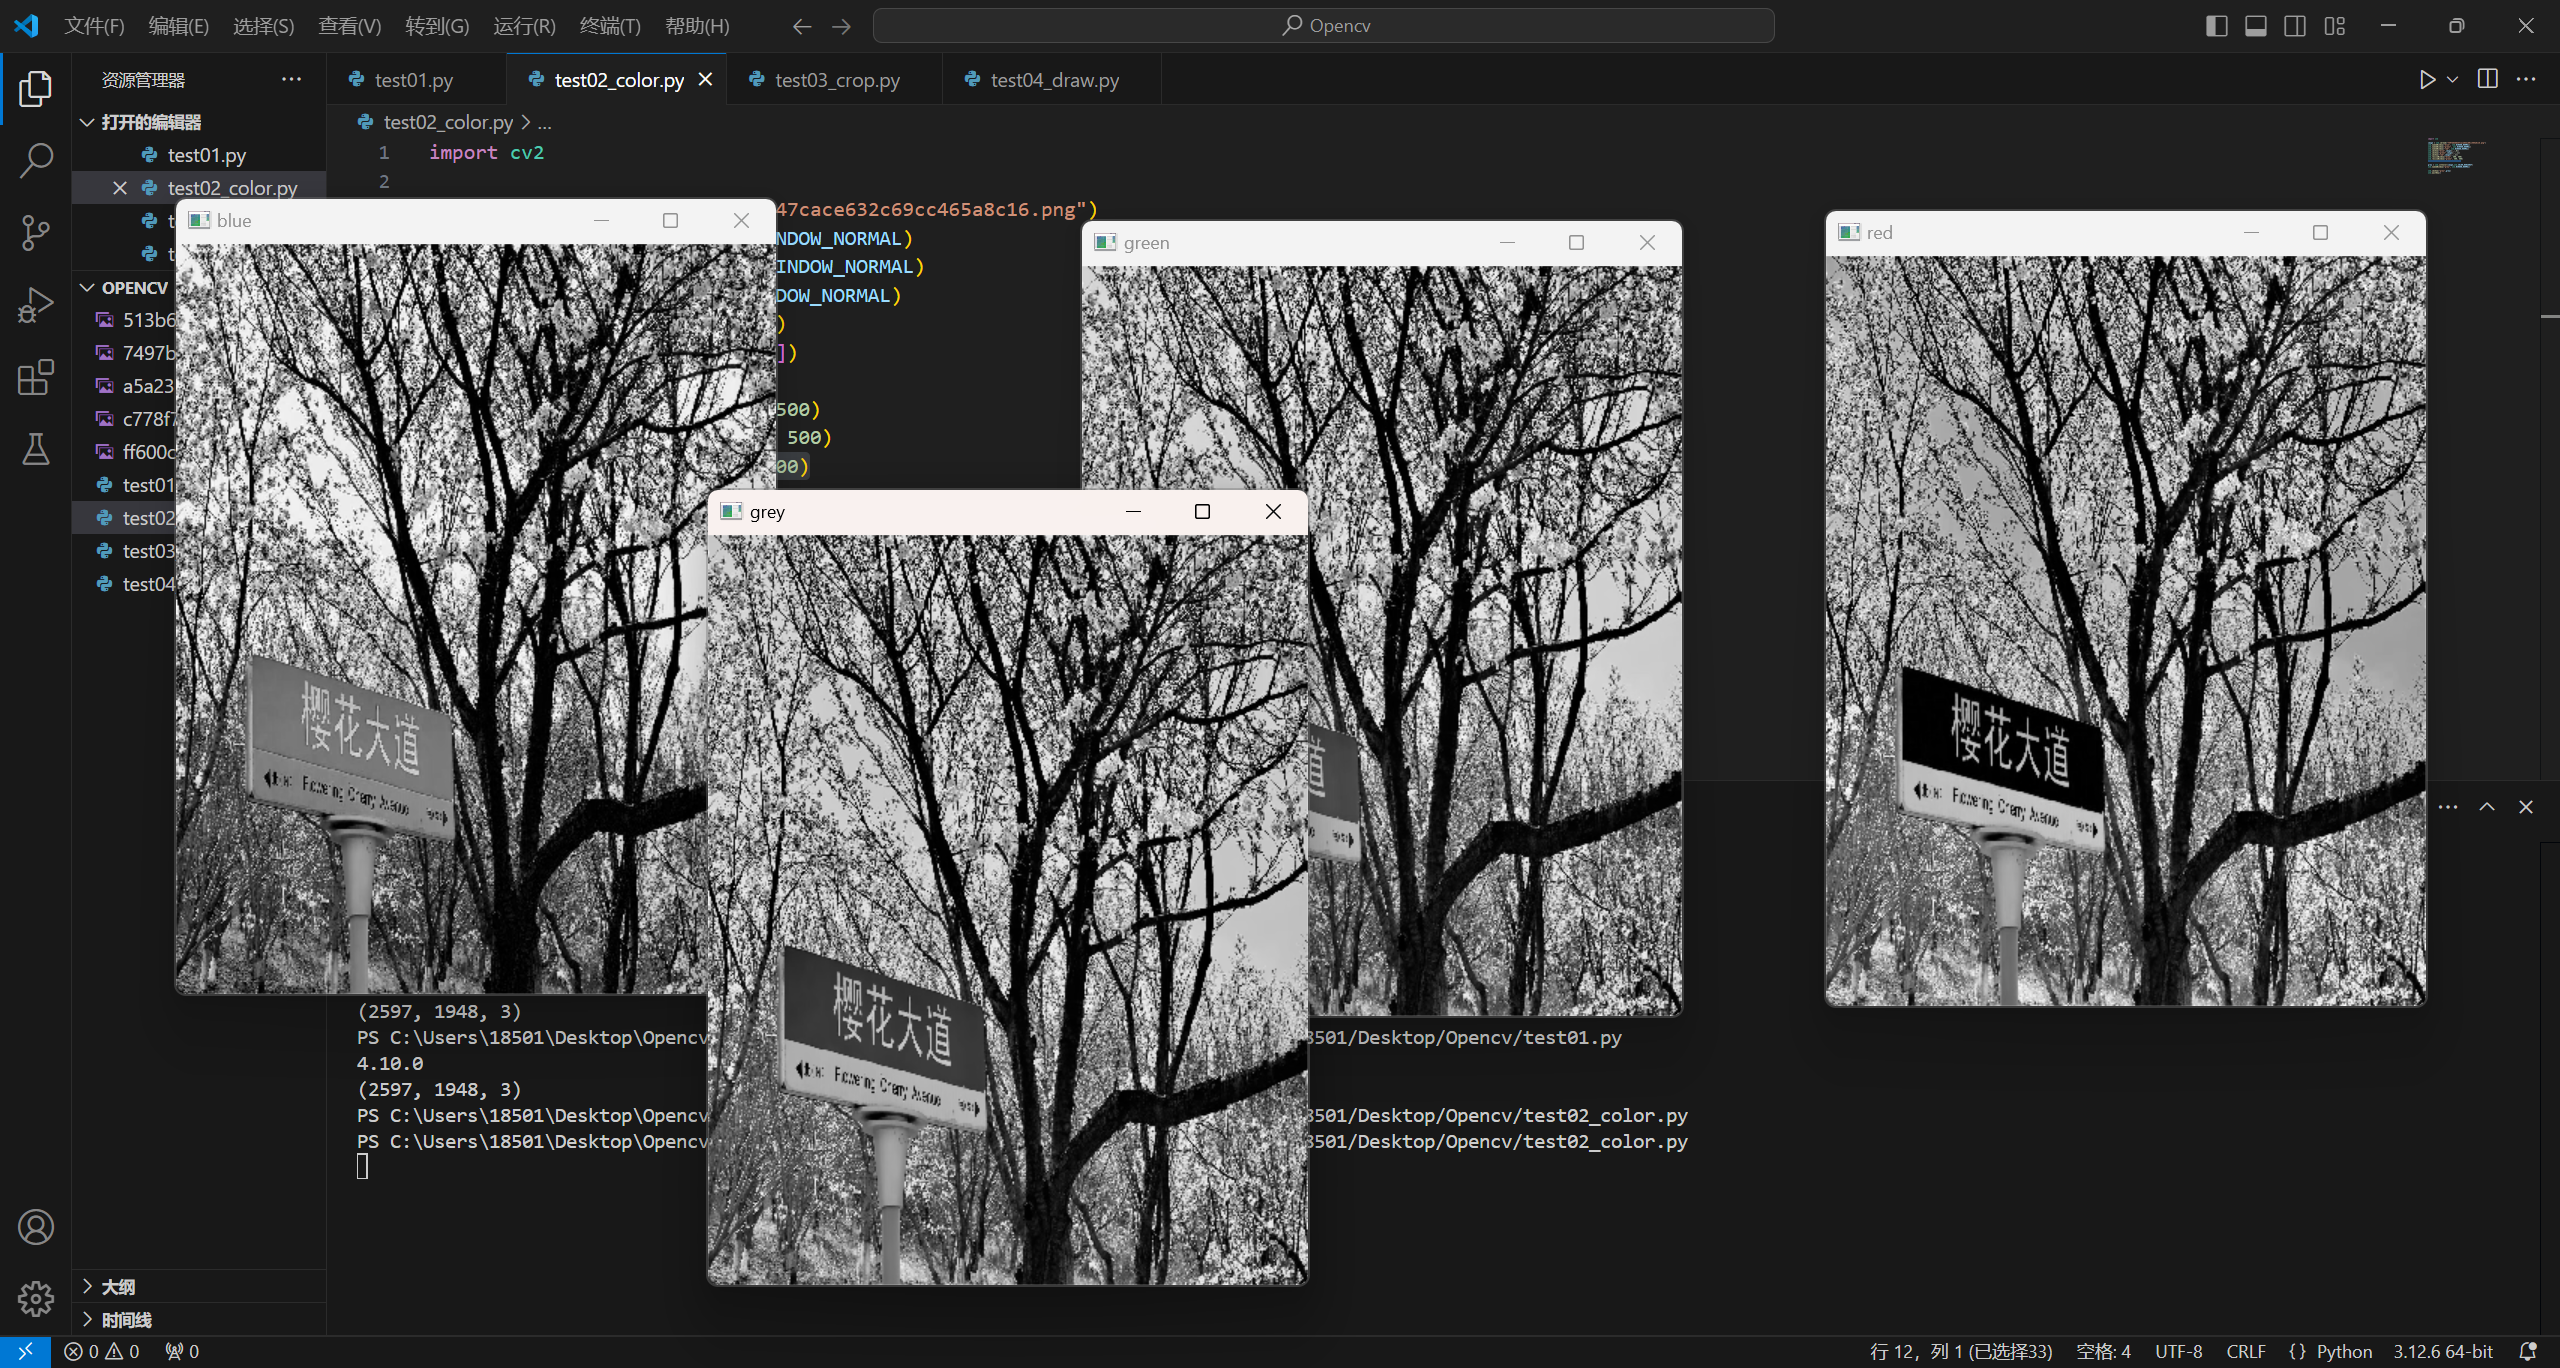
\includegraphics[width=14cm]{094f5864a7ce86daf98420c76f9ead6e.png}
        \caption{灰度图运行结果}
        \label{fig:1}
    \end{figure}
    \item 绘制图片(线段,图形,文字)
    \begin{figure}[H]
        \centering
        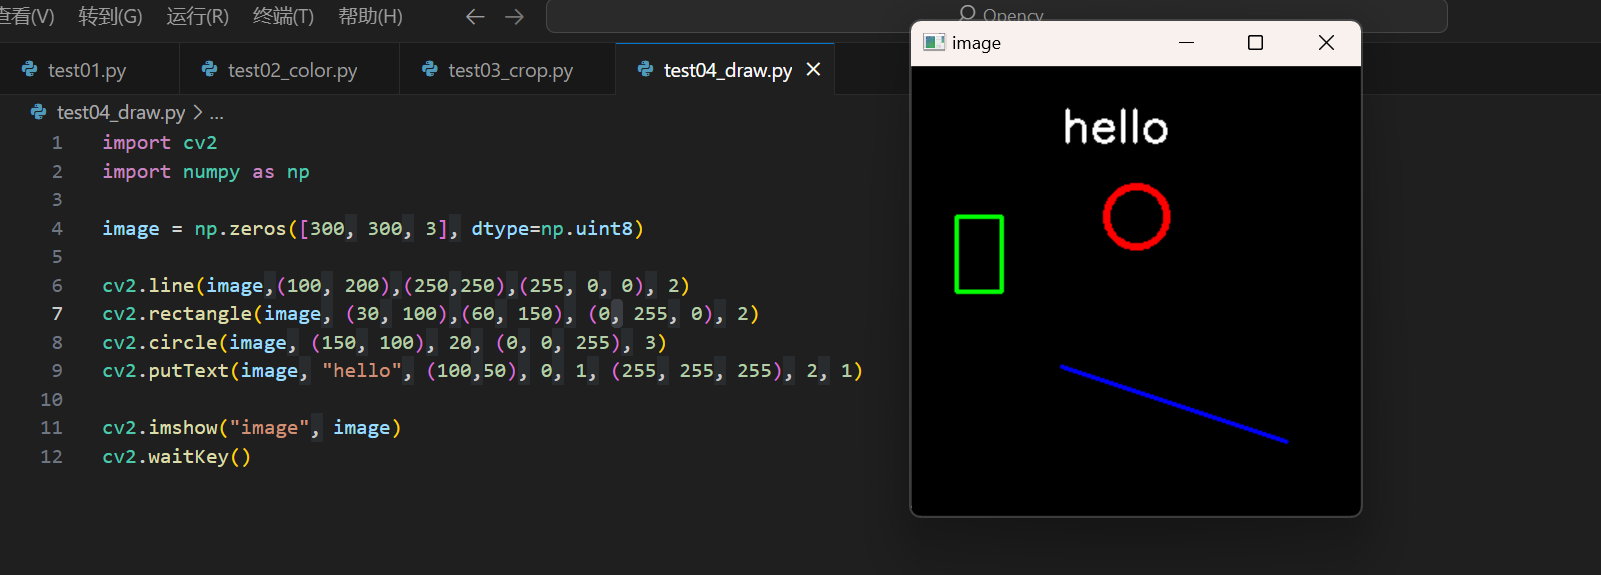
\includegraphics[width=14cm]{6c4f6d14ca5d99347b941438aaf626ac.png}
        \caption{代码及运行效果}
        \label{fig:1}
    \end{figure}
\end{enumerate}

\section{实验心得}
\subsection{学习命令行环境}

命令行环境提供了一种直接与操作系统交互的高效方式。通过学习命令行,我深刻体会到它的强大和灵活性。能够熟练使用各种命令来进行文件操作、进程管理等,让我对计算机系统的底层运作有了更深入的理解。它就像是掌握了一把开启系统奥秘的钥匙,让我可以更快捷、精准地完成各种任务,同时也为后续更复杂的编程和技术学习奠定了坚实的基础。

\subsection{Python入门基础}

学习 Python 入门基础是一段充满新奇和挑战的旅程。我明白了 Python 简洁易懂的语法是其魅力所在,它让编程变得不再那么遥不可及。在学习过程中,逐渐掌握了变量、数据类型、控制结构等基础知识,能够用代码表达自己的想法和逻辑。通过编写简单的程序,不断积累经验,也培养了逻辑思维和问题解决能力。而且 Python 拥有丰富的库和工具,为进一步探索各种应用领域提供了广阔的空间。

\subsection{Python视觉应用}

探索 Python 视觉应用让我看到了编程在图像和视频处理领域的巨大潜力。学习过程中,了解到如何利用相关的库和算法来实现图像的读取、处理、分析和可视化。这不仅开拓了我的视野,还让我感受到了技术与艺术的结合。通过实际操作,我能够亲身体验到如何从原始的图像数据中提取有价值的信息,并且可以创造出有趣的视觉效果。同时,也意识到在这个领域需要不断学习新的知识和算法,以跟上技术的发展步伐。\\

总的来说,学习这些内容让我在技术的世界里不断成长和进步,每一个阶段都有独特的收获和感悟。
\section{Github仓库ssh链接}
 \url {git@github.com:xixiyhaha/psychic-octo-engine.git }
\end{document}